\documentclass{jsarticle}
\usepackage{moreverb}
\usepackage[dvipdfmx]{graphicx, hyperref}
\usepackage{float}
\usepackage{amsmath}
\usepackage{amssymb}

\usepackage{atbegshi}
\ifnum 42146=\euc"A4A2 \AtBeginShipoutFirst{\special{pdf:tounicode EUC-UCS2}}\else
\AtBeginShipoutFirst{\special{pdf:tounicode 90ms-RKSJ-UCS2}}\fi

%\bibliographystyle{junsrt}


\title{計算機実習 問題14.8 迷路の蟻}
\author{早稲田大学先進理工学部物理学科 B4 藤本將太郎}
\date{\today}

\begin{document}
    図5の結果を両対数グラフで表し,$D_{s}(p)=(p-p_{c})^{\mu_{s}}$であるとしてフィッティングし,$\mu_{s}$を求めた.
    \begin{figure}[H]
        \begin{center}
            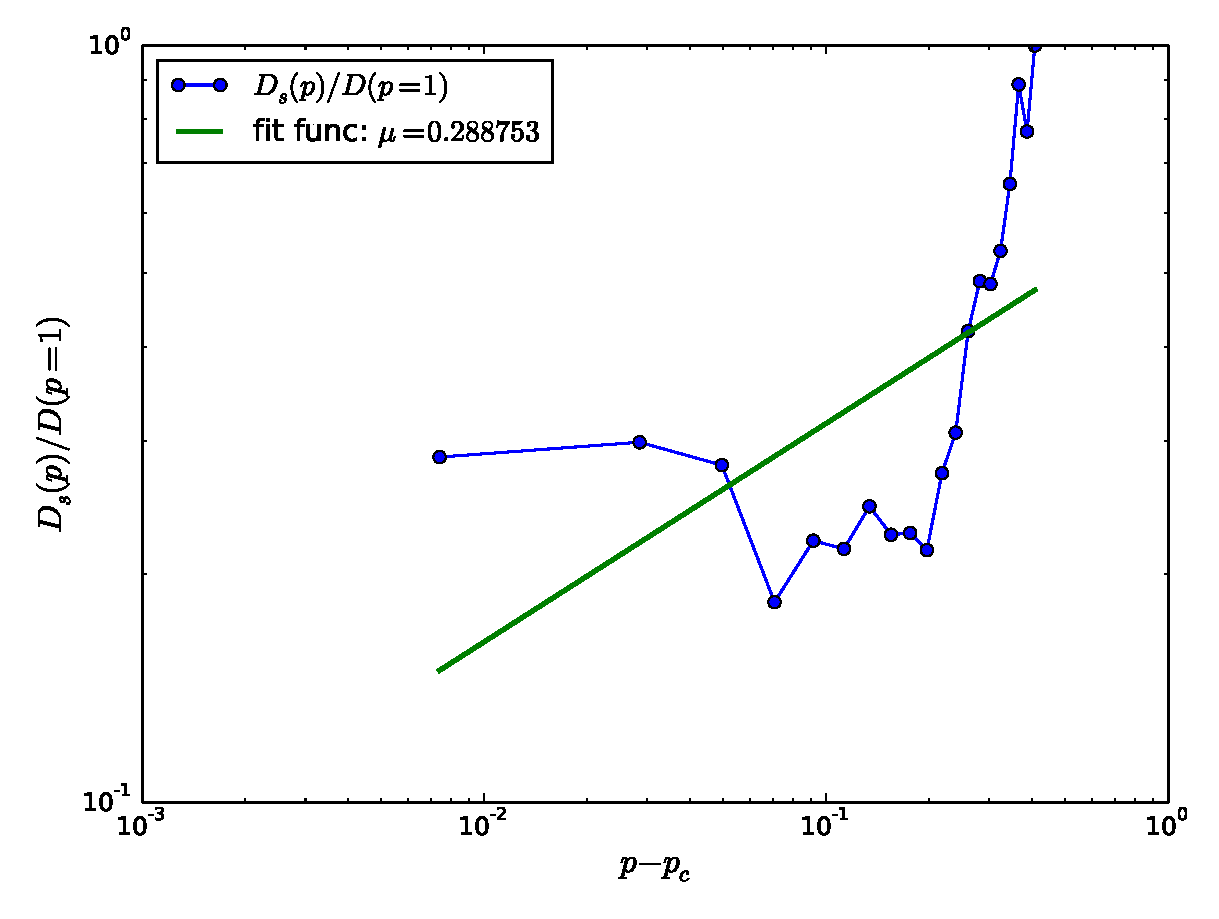
\includegraphics[width=10.0cm]{figure_8.pdf}
            \caption{図5のすべての結果を用いた場合の両対数グラフ}
        \end{center}

    \end{figure}

    \begin{figure}[H]
        \begin{center}
            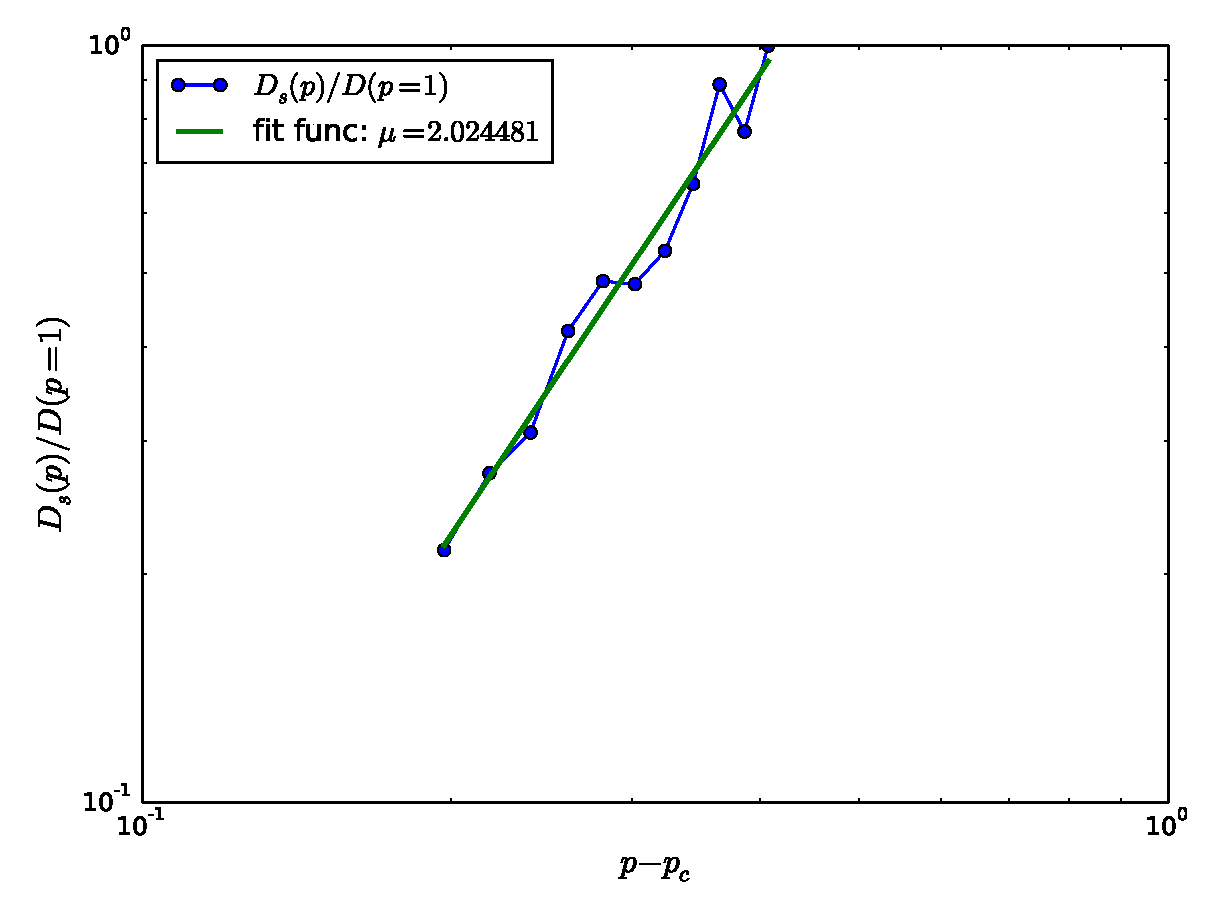
\includegraphics[width=10.0cm]{figure_9.pdf}
            \caption{図5の一部を用いた場合の両対数グラフ}
        \end{center}
        図から$p$の大きいところのデータを用いて得られた指数$\mu_{s}$は$\mu_{s}=2.024481$と求められた.
    \end{figure}
        


%\nocite{textbook}
%\nocite{fractal1}
%\bibliography{/home/shotaro/Workspace/computing_simulation/reference}


\end{document}
